L'exercice 4.1 du syllabus d'exercices a été implémenté dans le projet de sorte à valider mon simulation de raytracing. Pour ce faire, j'ai redéfini l'environnement en respectant les dimensions de l'exercice et j'ai également placé un émetteur en (32;10) et un récepteur en (47;65). La fréquence utilisée est de 868.3 MHz. Le seuil de sensibilité du récepteur est de -65 dBm.


Afin d'assurer le bon fonctionnement de tous les cas différents, incluant la propagation directe, la réflexion simple, la double réflexion et la transmission, les valeurs obtenues ont été reprises et comparées aux résultats de la simulation. Les rayons ont également été dessinés pour s'assurer que la correspondance avec les résultats attendus soit exacte et que tout soit correct. \footnote{Tous les graphes de ce chapitre sont en grande taille en Annexe A.}


\section{Equations générales pour les différents cas}
La propagation directe peut être modélisée par l'équation suivante:
\begin{equation}
\underline{E_n} = \Gamma_1 \Gamma_2 \Gamma_3 \ldots T_1 T_2 T_3 \ldots \sqrt{60 G_{TX}(\theta_{TX_n},\phi_{TX_n}) P_{TX}} \frac{e^{-j\beta d_n}}{d_n}
\end{equation}
où $\Gamma_i$ et $T_i$ représentent respectivement les coefficients de réflexion et de transmission.

\subsubsection{Puissance reçue}
La puissance reçue par le récepteur est donnée par l'équation suivante:
\begin{equation}
P_{RX} = \frac{1}{8Ra} \left|\sum_{n=1}^{N} \vec{h_e^{RX}}\left(\frac{\pi}{2}, \phi_n\right) \underline{E_n}(\vec{r})\right|^2
\end{equation}
$\theta = \frac{\pi}{2}$ est utilisé pour les calculs, car une adaptation parfaite et une polarisation perpendiculaire sont supposées.

\subsubsection{Impédance du mur et constante de propagation }
L'impédance du mur et la constante de propagation sont calculées à l'aide des formules suivantes, en considérant les propriétés électromagnétiques des matériaux:
\begin{align}
Z_m &= \sqrt{\frac{\mu_0}{\epsilon - j\sigma/\omega}} \approx (171.57 + j6.65) \, \Omega, \\
\gamma_m &= \alpha_m + j\beta_m = 1.55 + j39.90.
\end{align}
Ensuite les différents coefficients et angles dépendent du type de réflexions avec un obstacle et vont être comparés ci dessous.

\section{Visualisations et Comparaisons manuscrites et du simulateur}
\subsubsection{Visualisations}

Tout d'abord voici les tracés de rayons réalisés par le simulateur. Ceux-ci sont similaires à ceux de l'exercice du syllabus dont les tracés ne seront pas repris ici.
\begin{figure}[H]
\centering
\begin{subfigure}[b]{0.42\textwidth}
    \centering
    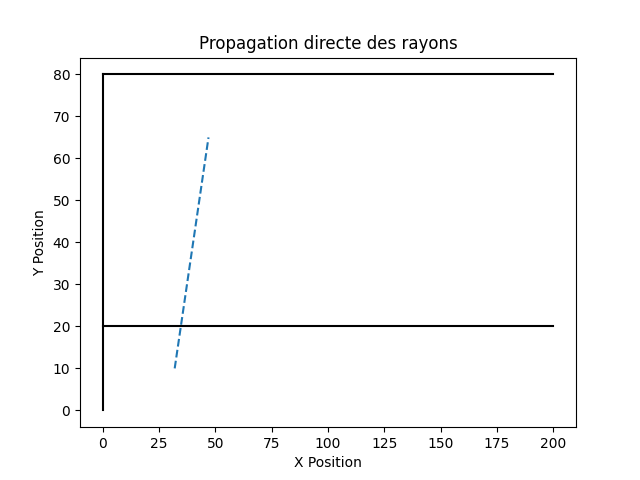
\includegraphics[width=\textwidth]{Pictures/propa_dir.png}
    \caption{Propagation directe \ref{fig:propd}}
    \label{fig:direct1}
\end{subfigure}
\hfill
\begin{subfigure}[b]{0.5\textwidth}
    \centering
    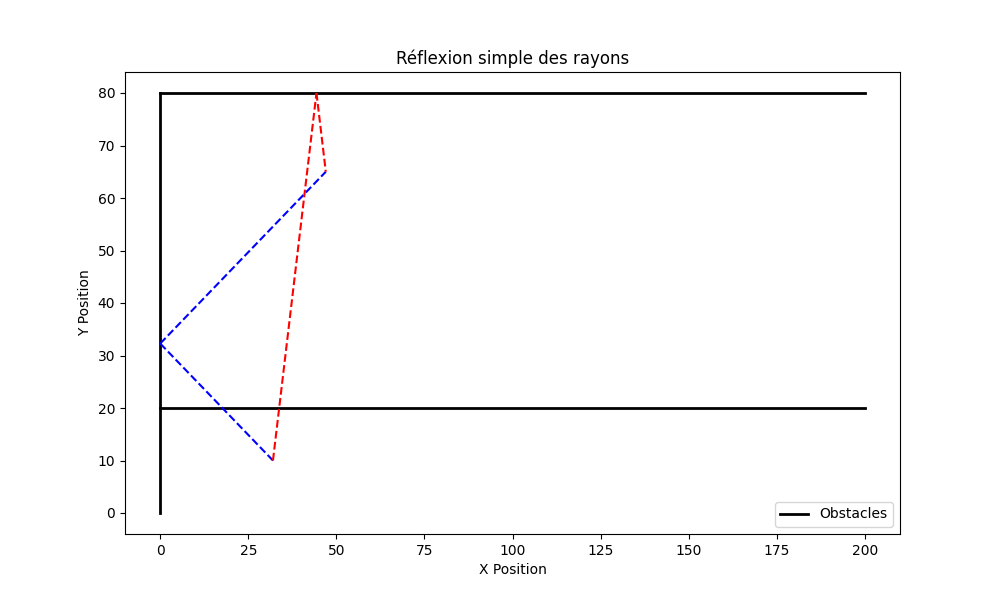
\includegraphics[width=\textwidth]{Pictures/simple_reflex.png}
    \caption{Réflexion simple \ref{refs}}
    \label{fig:simple_reflection}
\end{subfigure}

\begin{subfigure}[b]{0.45\textwidth}
    \centering
    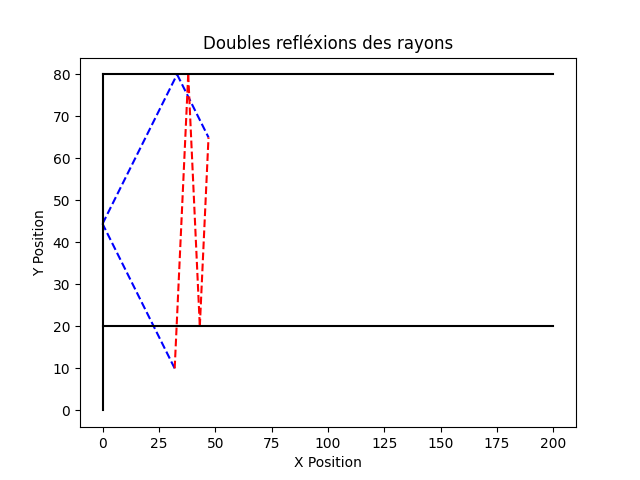
\includegraphics[width=\textwidth]{Pictures/double_reflex.png}
    \caption{Double réflexions \ref{refd}}
    \label{fig:double_reflection}
\end{subfigure}
\caption{Comparaison des différents types de propagation.}
\label{fig:ray_tracing}
\end{figure}

\subsubsection{Comparaison des Résultats}
Ci-dessous, le tableau comparant les valeurs obtenues manuellement avec celles de la simulation pour la propagation directe \ref{fig:direct1}.
\begin{table}[htbp]
\centering
\caption{Comparaison des résultats manuels et de simulation pour la propagation directe}
\label{tab:comparaison}
\begin{tabular}{@{}lcc@{}}
\toprule
\textbf{Paramètre} & \textbf{Valeur Manuelle} & \textbf{Valeur de Simulation} \\ \midrule
Champs Electrique (V/m) & $0.0037-0.0016j$ & $-0.0039994+3.8172944\times 10^{-5}j$ \\
Puissance reçue (W) &  $3.33 \times 10^{-10}$& $3.308468 \times 10^{-10}$ \\
Coefficient de transmission & $0.69+0.23j$ & $0.689195 + 0.237003j$ \\
Distance additionnelle parcourue (m) & $0.151$ & $0.151094$ \\
Angle d'incidence (degrés) & $15.2551$ & $15.255119$ \\
Angle de transmission (degrés) & $6.8796$ & $6.897650$ \\
Gamma perpendiculaire & $-0.3862+0.0165j$ & $-0.385931 + 0.016510j$ \\
$\gamma_m$ & $1.55+39.90j$ & $1.547482 + 39.872766j$ \\
Impédance du matériau $(\Omega)$ &$171.57+6.65j$& $171.683875 + 6.663138j$ \\
\bottomrule
\end{tabular}
\end{table} \\
La comparaison peut également être faite avec le cas à une réflexion pour le cas A (cas en bleu sur le graphe de la refléxion simple \ref{fig:simple_reflection}).
\begin{table}[htbp]
\centering
\caption{Comparaison des résultats manuels et de simulation pour la réflexion simple cas A}
\label{tab:comparaison_reflection}
\begin{tabular}{@{}lcc@{}}
\toprule
\textbf{Paramètre} & \textbf{Valeur Manuelle} & \textbf{Valeur de Simulation} \\ \midrule
Point d'impact ($P_r$) & $(0.0; 32.28)$ & $(0.0, 32.278481)$ \\
Angle d'incidence (degrés) & $34.8199$ & $34.84573$ \\
Angle de transmission (degrés) & $15.129$ & $15.1171208$ \\
Gamma perpendiculaire &$-0.4416+0.0156j$&$-0.441361+0.0156203j$\\
Coefficient de réflexion & $-0.334+0.225j$ & $-0.335708 + 0.225861j$ \\
Point d'impact ($P_t$) & $(17.64; 20)$ & $(17.636363;20)$ \\
Angle d'incidence (degré) & $55.1758$ & $55.1542665$ \\
Coefficient de transmission 1 (Émetteur $\rightarrow P_r$) & $0.539+0.023j$ & $0.537694 + 0.024983j$ \\
Distance additionnelle 1 (m) & $0.162$ & $0.161779$ \\
Coefficient de transmission 2 ($P_r \rightarrow$ récepteur) & $1+0j$ & $1.000000 + 0.000000j$ \\
Distance additionnelle 2 (m) & $0$ & $0.000000$ \\
Champs Electrique (V/m) & $-5.41\times 10^{-4}-4.57\times 10^{-4}j$ & $0.000441355+0.00055429153j $\\
Puissance reçue (W) &  $10.4 \times 10^{-12}$& $1.03829831227 \times 10^{-11}$ \\
\bottomrule
\end{tabular}
\end{table}\\
Pour les cas B à une reflexion et deux réflexion les résultats obtenus sont également ci dessous.\\
\begin{table}[H]
\centering
\caption{Comparaison des résultats manuels et de simulation pour les réflexions simple et doubles cas B}
\label{tab:comparaison_reflection}
\begin{tabular}{@{}lcc@{}}
\toprule
\textbf{Paramètre} & \textbf{Valeur Manuelle} & \textbf{Valeur de Simulation} \\ \midrule
cas B, réflexion simple & &\\ 
Champs Electrique (V/m) & $-4.52\times 10^{-4}-5.06\times 10^{-4}j$ & $0.000672792+0.00010809859j $\\
Puissance reçue (W) &  $9.5 \times 10^{-12}$& $9.6033123939 \times 10^{-12}$ \\
cas B, réflexion double & &\\ 
Champs Electrique (V/m) & $-7.86\times 10^{-5}-5.19\times 10^{-6}j$ & $-2.3403616\times 10^{-5} -7.614057941\times 10^{-5}j $\\
Puissance reçue (W) &  $0.1 \times 10^{-12}$& $1.3122870783 \times 10^{-13}$ \\
\bottomrule
\end{tabular}
\end{table}\\

Il est important de noter que les champs électriques sont différent pour les différents cas mais cela est dû à la grande variation de phase car l'émetteur est à $868.3 MHz$.\\
Après comparaison avec l'exercice 4.1 du syllabus du cours, les résultats sont similaire. Le simulateur est donc vérifié.
\section{Calcul du cas à 2 réflexions cas A}
Il a été demandé de calculer l'un des deux cas à 2 réflexions. Le cas ci dessous sera donc étudié.  
\begin{figure}[H]
    \centering
    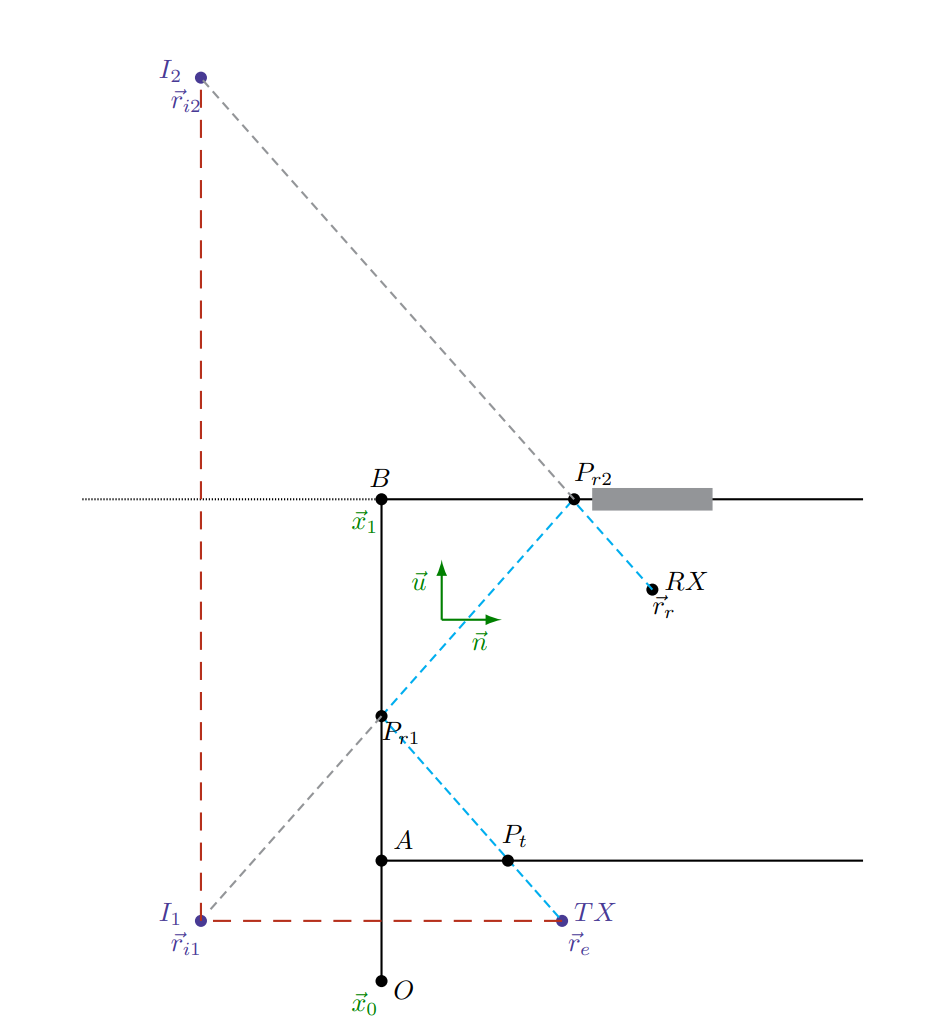
\includegraphics[width=0.58\textwidth]{Pictures/ex41.png}
    \caption{Cas A à 2 réflexions exercice 4.1}
    \label{fig:enter-label}
\end{figure}
\section*{Calcul des positions des points $Pr_2$, $Pr_1$ et $Pt$}

La position des antennes images est déterminée par symétrie orthogonale, avec les coordonnées suivantes pour les antennes images : $I_1 = (-32, 10)$ et $I_2 = (-32, 150)$. Les coordonnées des points $Pr_2$, $Pr_1$ et $Pt$ sont calculées comme suit :


\subsection*{Calcul de $Pr_2$}
$Pr_2$ est un point intermédiaire sur le trajet reliant $I_2$ à $RX$.Pour commencer, le vecteur a été calculé $\vec{v}_1$ entre $I_2$ et $RX$:
\[
\vec{v}_1 = (47 - (-32), 65 - 150) = (79, -85)
\]
La norme de $\vec{v}_1$ est calculée par :
\[
\|\vec{v}_1\| = \sqrt{79^2 + (-85)^2} = 116.0431
\]
Le vecteur unitaire de $\vec{v}_1$ est donc :
\[
\vec{u}_1 = \left(\frac{79}{116.0431}, \frac{-85}{116.0431}\right) = (0.6808, -0.7325)
\]
En posant la coordonnée y de $Pr_2$ à 80, en résolvant pour $\lambda$ dans l'équation suivante :
\[
(y; 80) = (-32; 150) + \lambda \vec{u}_1 \implies \lambda = \frac{80 - 150}{-0.7325} = 95.5631
\]
D'où :
\[
x = -32 + 95.5631 \times 0.6808 = 33.0593
\]
Ainsi, $Pr_2 = (33.0593, 80)$.

\subsection*{Calcul de $Pr_1$}
Pour calculer $Pr_1$, reliant $I_1$ à $Pr_2$, le vecteur $\vec{v}_2$ est :
\[
\vec{v}_2 = (33.0593 - (-32), 80 - 10) = (65.0593, 70)
\]
Sa norme est :
\[
\|\vec{v}_2\| = \sqrt{(65.0593)^2 + 70^2} = 95.5652
\]
Le vecteur unitaire est :
\[
\vec{u}_2 = \left(\frac{65.0593}{95.5652}, \frac{70}{95.5652}\right) = (0.6808, 0.7325)
\]
Pour une coordonnée x de $Pr_1$ à 0, j'ai trouvé $\lambda$ :
\[
(0; y) = (-32; 10) + \lambda \vec{u}_2 \implies \lambda = \frac{0 - (-32)}{0.6808} = 47.0035
\]
Donc :
\[
y = 10 + 47.0035 \times 0.7325 = 44.4301
\]
Finalement, $Pr_1 = (0, 44.4301)$.

\subsection*{Calcul de $Pt$}
La méthode similaire est appliquée pour $Pt$. Le vecteur $\vec{v}_3$ et sa norme sont :
\[
\vec{v}_3 = (0 - 32, 44.4301 - 10) = (-32, 34.4301), \quad \|\vec{v}_3\| = \sqrt{(-32)^2 + (34.4301)^2} = 47.0046
\]
Le vecteur unitaire est :
\[
\vec{u}_3 = \left(\frac{-32}{47.0046}, \frac{34.4301}{47.0046}\right) = (-0.6808, 0.7325)
\]
Pour une coordonnée y de $Pt$ à 20, $\lambda$ est résolu comme suit :
\[
(x; 20) = (32; 10) + \lambda \vec{u}_3 \implies \lambda = \frac{20 - 10}{0.7325} = 13.6519
\]
Ce qui donne :
\[
x = 32 + 13.6519 \times (-0.6808) = 22.7058
\]
Ainsi, $Pt = (22.7058, 20)$.

\section*{Coefficients de réflexion et transmission}

Le rayon subit une transmission et deux réflexions au cours de son trajet. Il est donc nécessaire de calculer deux coefficients de réflexion ainsi qu'un coefficient de transmission.

\subsection*{Calcul du coefficient $\Gamma_2$}
Le vecteur normal au point $Pr_2$ est donné par $(0, -1)$. La projection de $\vec{v}_1$ normé sur ce vecteur normal donne $\cos \theta_i = \langle (0.6808, -0.7325), (0, -1) \rangle = 0.7325$. Ainsi, $\sin \theta_i$ est obtenu par:
\[
\sin \theta_i = \sqrt{1 - 0.7325^2} = 0.6808.
\]
Le $\sin \theta_t$ est déterminé par la loi de Snell:
\[
\sin \theta_t = \sqrt{\frac{1}{\epsilon_r}} \sin \theta_i = \sqrt{\frac{1}{4.8}} \times 0.6808 = 0.3107 \quad \text{et donc} \quad \cos \theta_t = \sqrt{1 - 0.3107^2} = 0.9505.
\]
La distance de pénétration $s$ est calculée comme:
\[
s = \frac{l}{\cos \theta_t} = \frac{0.15}{0.9505} = 0.1578.
\]
Le coefficient de réflexion $\Gamma_{\perp}$ est alors:
\[
\Gamma_{\perp} = \frac{Z_m \cos \theta_i - Z_0 \cos \theta_t}{Z_m \cos \theta_i + Z_0 \cos \theta_t} = \frac{(171.57 + j6.65) \times 0.7325 - 377 \times 0.9505}{(171.57 + j6.65) \times 0.7325 + 377 \times 0.9505} = -0.4805 + j0.0149.
\]
Avec ces valeurs, $\Gamma_2$ est calculé par:
%\Gamma_m(\theta_i) = \Gamma_{\perp}(\theta_i) - \frac{(1 - \Gamma^2_{\perp}(\theta_i)) \Gamma_{\perp}(\theta_i) e^{-2\gamma_m s} e^{j\beta2s \sin \theta_t \sin \theta_i}}{1 - \Gamma^2_{\perp}(\theta_i) e^{-2\gamma_m s} e^{j\beta2s \sin \theta_t \sin \theta_i}}

\[
\Gamma_2 =  \Gamma_{\perp}(\theta_i) -(1 - \Gamma^2_{\perp}(\theta_i)) \frac{ \Gamma_{\perp}(\theta_i) e^{-2\gamma_m s} e^{j\beta2s \sin \theta_t \sin \theta_i}}{1 - \Gamma^2_{\perp}(\theta_i) e^{-2\gamma_m s} e^{j\beta2s \sin \theta_t \sin \theta_i}} = -0.4188 + 0.2462j.
\]

\subsection*{Calcul du coefficient $\Gamma_1$}
Pour le deuxième calcul, je projete $\vec{v}_2$ normé sur la normale $(1, 0)$, donnant $\cos \theta_i = 0.6808$. Les calculs suivants utilisent cette valeur:
\[
\sin \theta_i = 0.7325, \quad \sin \theta_t = 0.3343, \quad \cos \theta_t = 0.9425, \quad s = 0.1591.
\]
Le coefficient de réflexion perpendiculaire $\Gamma_a$ est:
\[
\Gamma_{a,\perp} = \frac{Z_m \cos \theta_i - Z_0 \cos \theta_t}{Z_m \cos \theta_i + Z_0 \cos \theta_t} = \frac{(171.57 + j6.65) \times 0.6808 - 377 \times 0.9425}{(171.57 + j6.65) \times 0.6808 + 377 \times 0.9425} = -0.5050 + j0.0144.
\]
Ainsi, $\Gamma_1$ est:
\[
\Gamma_1 = \Gamma_{\perp}(\theta_i) -(1 - \Gamma^2_{\perp}(\theta_i)) \frac{ \Gamma_{\perp}(\theta_i) e^{-2\gamma_m s} e^{j\beta2s \sin \theta_t \sin \theta_i}}{1 - \Gamma^2_{\perp}(\theta_i) e^{-2\gamma_m s} e^{j\beta2s \sin \theta_t \sin \theta_i}}= -0.4710 + 0.2518j.
\]

\subsection*{Calcul du coefficient de transmission $T_1$}
Le $\cos \theta_i$ pour le point $Pt$ est $0.7325$. En dérivant $\sin \theta_i$, $\sin \theta_t$, et $\cos \theta_t$ comme précédemment. Le coefficient de réflexion perpendiculaire $\Gamma_b$ est:
\[
\Gamma_{b,\perp} = \frac{Z_m \cos \theta_i - Z_0 \cos \theta_t}{Z_m \cos \theta_i + Z_0 \cos \theta_t} = \frac{(171.57 + j6.65) \times 0.7325 - 377 \times 0.1578}{(171.57 + j6.65) \times 0.7325 + 377 \times 0.1578} = -0.5082 + j0.0144.
\]
Le coefficient de transmission $T_1$ est alors calculé par:
\[
T_1 = \frac{ (1 - \Gamma^2_{\perp}(\theta_i)) e^{-2\gamma_m s}}{1 - \Gamma^2_{\perp}(\theta_i) e^{-2\gamma_m s} e^{j\beta2s \sin \theta_t \sin \theta_i}} = 0.6295 + 0.0890j.
\]

%\section*{Calcul de la distance totale parcourue par le rayon et puissance reçue au récepteur}

%\subsection*{Distance totale parcourue par le rayon}
%La distance totale parcourue par le rayon est calculée en additionnant les distances entre les différents points du trajet du rayon de $TX$ à $RX$ :
%\begin{align*}
%\text{Trajet } TX/Pt & : \sqrt{(22.7058 - 32)^2 + (20 - 10)^2} = 13.6522, \\
%\text{Trajet } Pt/Pr1 & : \sqrt{(0 - 22.7058)^2 + (44.4301 - 20)^2} = 33.3524, \\
%\text{Trajet } Pr2/Pr1 & : \sqrt{(33.0593 - 0)^2 + (80 - 44.4301)^2} = 48.5606, \\
%\text{Trajet } PRX/Pr2 & : \sqrt{(47 - 33.0593)^2 + (65 - 80)^2} = 20.4779.
%\end{align*}
%La distance totale est donc de $116.0431$ mètres. Cette distance peut également être vérifiée en calculant directement la distance entre la dernière antenne image $I_2$ et le récepteur $RX$ :
%\[
%\sqrt{(47 - (-32))^2 + (65 - 150)^2} = 116.0431 \text{ mètres}.
%\]

\subsection{Calcul du champ et de la puissance reçue au récepteur}
La valeur du champ électrique reçu, $E_n$, est calculée à partir des coefficients de transmission et de réflexion, et est donnée par :
\[
E_n = \Gamma_1 \Gamma_2 T_1 \sqrt{60 G_{TX} P_{TX}} \frac{e^{-j \beta d_n}}{d_n}
\]
où $\Gamma_1 = -0.4710 + 0.2518j$, $\Gamma_2 = -0.4188 + 0.2462j$, $T_1 = 0.6295 + 0.0890j$, et $d_n = 116.0431$(norme de $v_1$). En calculant $\Gamma_1 \Gamma_2 T_1$ :
\[
\Gamma_1 \Gamma_2 T_1 = (-0.4710 + 0.2518j)(-0.4188 + 0.2462j)(0.6295 + 0.0890j) = 0.1059 - 0.1273j
\]
Ainsi, en substituant les valeurs et calculant $\beta$ à partir de la fréquence $f = 868.3$ MHz :
\[
\beta = \frac{2\pi f}{c} = \frac{2\pi \times 868.3 \times 10^6}{3 \times 10^8} \quad (\text{avec } c \text{ la vitesse de la lumière})
\]
La valeur de $E_n$ obtenue est :

\[
E_n = (0.0159 - 0.1273j) \sqrt{60 \times 1.64 \times 10^{-3}} \frac{e^{-j \beta \times 116.0431}}{116.0431} 
\]
\[
E_n \approx 4.4519 \times 10^{-4} - 2.1816 \times 10^{-5}j
\]
La puissance totale reçue, $P_{RX}$, est ensuite calculée par :
\[
P_{RX} = \frac{\lambda^2}{8\pi^2 R_a} \|E_n\|^2 = \left(\frac{3 \times 10^8}{868.3 \times 10^6}\right)^2 \frac{1}{8\pi^2 \times 73} \|4.4519 \times 10^{-4} - 2.1816 \times 10^{-5}j\|^2
\]
\[
P_{RX} \approx 4.1145 \times 10^{-12} \text{ Watts} \quad \text{ou} \quad P_{RX} \approx -83.8568 \text{ dBm}
\]
\begin{table}[htbp]
\centering
\caption{Comparaison des résultats manuels et simulés pour la réflexion doubles cas A}
\label{tab:double_reflection_comparison}
\begin{tabular}{@{}lcc@{}}
\toprule
\textbf{Paramètre} & \textbf{Valeur Manuelle} & \textbf{Valeur de Simulation} \\ \midrule
Point d'impact 1 & $(0, 44.4301)$ & $(0.0, 44.4304)$ \\
Point d'impact 2 & $(33.0593, 80)$ & $(33.059, 80.0)$ \\
Angle d'incidence($\Gamma_1$) $\theta_{i1}$ (degrés) & $47.09381$ & $47.09525256$ \\
Angle de transmission $\theta_t1$ (degrés) & $19.531$ & $19.531971$ \\
Angle d'incidence($\Gamma_2$) $\theta_{i2}$ (degrés) & $42.9031$ & $42.90474743$ \\
Angle de transmission $\theta_t2$ (degrés) & $18.103$ & $18.1034009$ \\
Coefficient de réflexion $\Gamma_{\perp1}$ & $(-0.5050+0.0144j)$ & $(-0.504537+0.014614j)$ \\
Coefficient de réflexion $\Gamma_{\perp2}$ & $(-0.4805+0.0149j)$ & $(-0.480021+0.014929j)$ \\
Coefficients de transmission 1 & $(0.6295+0.0890j)$ & $(0.6289223+0.0918245j)$ \\
Coefficients de transmission 2 & $1.0$ & $1.0$ \\
Coefficients de transmission 3 & $1.0$ & $1.0$ \\
Distance totale (mètres) & $116.0431$ & $116.043095$ \\
Coefficient total & $(0.1059-0.1273j)$ & $(0.1064106-0.1273762j)$ \\
Champ électrique (V/m)& $4.4519 \times 10^{-4} - 2.1816 \times 10^{-5}j$ & $(3.05628 \times 10^{-5} - 0.0004476j)$  \\
Puissance reçue (W)&$4.1145 \times 10^{-12}$ & $4.16327 \times 10^{-12}$  \\

\bottomrule
\end{tabular}
\end{table}
